\subsection{Methods}
\subsubsection{More about Haar feature-based cascade classifier}
We use a Haar features-based cascade to detect the face.
\begin{figure}[ht]
	\centering		
	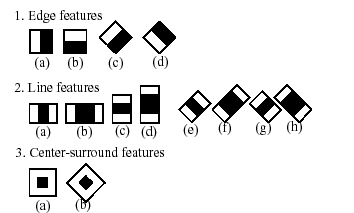
\includegraphics[width = 0.4\textwidth]{rsrc/Haarfeatures.png}
	\caption{Haar features used in openCV (including 45° features)}
	\label{fig:Haar features}
\end{figure}
The output will be the difference between the sum of the intensities on the whole picture and the intensities on the black part of the feature. The features are scaled and move across the initial image. These are quickly calculated by using the corresponding intensity image.
\begin{figure}[ht]
	\centering		
	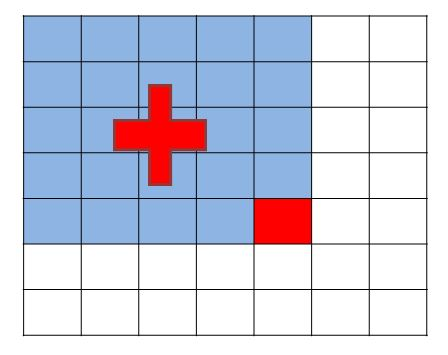
\includegraphics[width = 0.2\textwidth]{rsrc/IntegralImage.jpg}
	\caption{Integral image : sum of the intensities of the value of left and up pixels of the current pixel}
	\label{fig:Integral image}
\end{figure}
We use two intensity images, one adding the left and top pixels of the analysed pixel and an other intensity image adding the pixels in the corner of the current pixel made by two 45° lines.
The cascade is then trained. Adaboost is used for this purpose on positive images (a face, an eye, a nose, a mouth). The result is a sequences of criteria of recognition following a cascade checking of the object.
\begin{figure}[ht]
	\centering		
	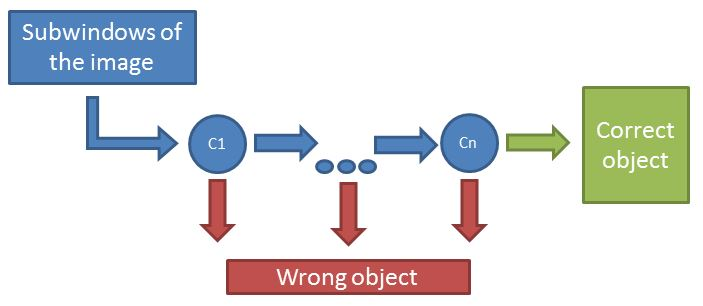
\includegraphics[width = 0.4\textwidth]{rsrc/Cascade.jpg}
	\caption{Cascade}
	\label{fig:Cascade}
\end{figure}



\subsubsection{Local Binary Pattern Histogram}

Computing of the new value of the central pixel, being the sum of powers of two combined with the value of the neighbours taken clockwise.
\begin{figure}[ht]
\centering
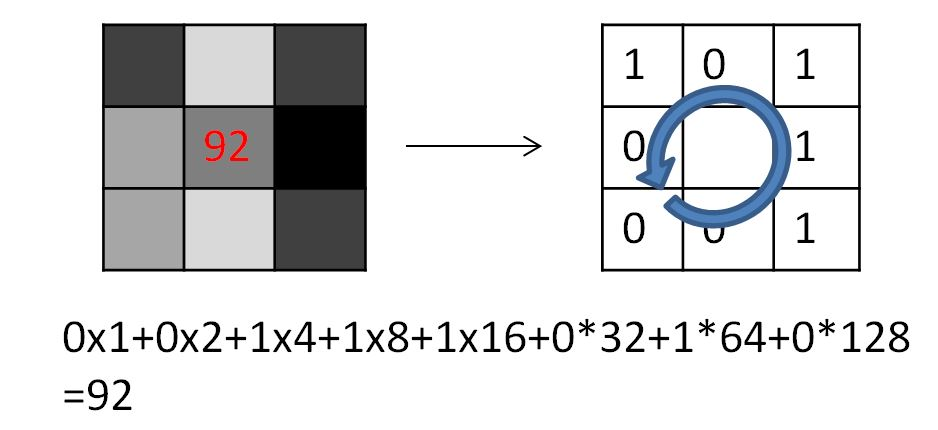
\includegraphics[width=2.5in]{rsrc/LBPH1.jpg}
\caption{Analysing the local structure}
\label{Local Structure}
\end{figure}

Addition of histograms from the subimages.

\begin{figure}[ht]
\centering
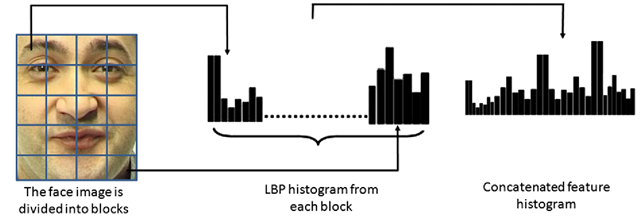
\includegraphics[width=2.5in]{rsrc/LBPH2.png}
\caption{Adding histograms (source : http://what-when-how.com/face-recognition/)}
\label{Adding histograms}
\end{figure}

\subsubsection{Neural Network}

The particularity of the feedback neural network is that some activation could have some impacts on previous nodes.
\begin{figure}[ht]
\centering
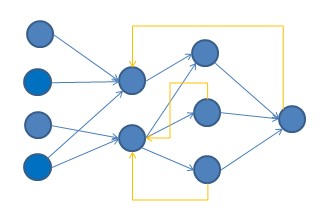
\includegraphics[width=2.5in]{rsrc/feedback_network.jpg}
\caption{Feedback Neural Network}
\label{Feedback Neural Network}
\end{figure}



%%\emph{Example of signifacance of patrial occlusion}
%%\title{Signifacance of patrial occlusion}
%%\subsection{\textbf{Signifacance of patrial occlusion}}
%%\begin{itemize}
%%	\item Eyes (occlusion of original image ~ 6\%)
%%	\item Eyebrows (occlusion of original image ~ 6\%)
%%	\item Mouth (occlusion of original image ~ 11\%)
%%	\item Eyes and nose (occlusion of original image ~ 9\%)
%%	\item Glasses (occlusion of original image ~ 15.5\%)
%%\end{itemize}


